% Options for packages loaded elsewhere
\PassOptionsToPackage{unicode}{hyperref}
\PassOptionsToPackage{hyphens}{url}
\PassOptionsToPackage{dvipsnames,svgnames,x11names}{xcolor}
%
\documentclass[
]{article}

\usepackage{amsmath,amssymb}
\usepackage{iftex}
\ifPDFTeX
  \usepackage[T1]{fontenc}
  \usepackage[utf8]{inputenc}
  \usepackage{textcomp} % provide euro and other symbols
\else % if luatex or xetex
  \usepackage{unicode-math}
  \defaultfontfeatures{Scale=MatchLowercase}
  \defaultfontfeatures[\rmfamily]{Ligatures=TeX,Scale=1}
\fi
\usepackage{lmodern}
\ifPDFTeX\else  
    % xetex/luatex font selection
\fi
% Use upquote if available, for straight quotes in verbatim environments
\IfFileExists{upquote.sty}{\usepackage{upquote}}{}
\IfFileExists{microtype.sty}{% use microtype if available
  \usepackage[]{microtype}
  \UseMicrotypeSet[protrusion]{basicmath} % disable protrusion for tt fonts
}{}
\makeatletter
\@ifundefined{KOMAClassName}{% if non-KOMA class
  \IfFileExists{parskip.sty}{%
    \usepackage{parskip}
  }{% else
    \setlength{\parindent}{0pt}
    \setlength{\parskip}{6pt plus 2pt minus 1pt}}
}{% if KOMA class
  \KOMAoptions{parskip=half}}
\makeatother
\usepackage{xcolor}
\usepackage[top=30mm,left=20mm,right=20mm,bottom=30mm]{geometry}
\setlength{\emergencystretch}{3em} % prevent overfull lines
\setcounter{secnumdepth}{5}
% Make \paragraph and \subparagraph free-standing
\makeatletter
\ifx\paragraph\undefined\else
  \let\oldparagraph\paragraph
  \renewcommand{\paragraph}{
    \@ifstar
      \xxxParagraphStar
      \xxxParagraphNoStar
  }
  \newcommand{\xxxParagraphStar}[1]{\oldparagraph*{#1}\mbox{}}
  \newcommand{\xxxParagraphNoStar}[1]{\oldparagraph{#1}\mbox{}}
\fi
\ifx\subparagraph\undefined\else
  \let\oldsubparagraph\subparagraph
  \renewcommand{\subparagraph}{
    \@ifstar
      \xxxSubParagraphStar
      \xxxSubParagraphNoStar
  }
  \newcommand{\xxxSubParagraphStar}[1]{\oldsubparagraph*{#1}\mbox{}}
  \newcommand{\xxxSubParagraphNoStar}[1]{\oldsubparagraph{#1}\mbox{}}
\fi
\makeatother

\usepackage{color}
\usepackage{fancyvrb}
\newcommand{\VerbBar}{|}
\newcommand{\VERB}{\Verb[commandchars=\\\{\}]}
\DefineVerbatimEnvironment{Highlighting}{Verbatim}{commandchars=\\\{\}}
% Add ',fontsize=\small' for more characters per line
\usepackage{framed}
\definecolor{shadecolor}{RGB}{241,243,245}
\newenvironment{Shaded}{\begin{snugshade}}{\end{snugshade}}
\newcommand{\AlertTok}[1]{\textcolor[rgb]{0.68,0.00,0.00}{#1}}
\newcommand{\AnnotationTok}[1]{\textcolor[rgb]{0.37,0.37,0.37}{#1}}
\newcommand{\AttributeTok}[1]{\textcolor[rgb]{0.40,0.45,0.13}{#1}}
\newcommand{\BaseNTok}[1]{\textcolor[rgb]{0.68,0.00,0.00}{#1}}
\newcommand{\BuiltInTok}[1]{\textcolor[rgb]{0.00,0.23,0.31}{#1}}
\newcommand{\CharTok}[1]{\textcolor[rgb]{0.13,0.47,0.30}{#1}}
\newcommand{\CommentTok}[1]{\textcolor[rgb]{0.37,0.37,0.37}{#1}}
\newcommand{\CommentVarTok}[1]{\textcolor[rgb]{0.37,0.37,0.37}{\textit{#1}}}
\newcommand{\ConstantTok}[1]{\textcolor[rgb]{0.56,0.35,0.01}{#1}}
\newcommand{\ControlFlowTok}[1]{\textcolor[rgb]{0.00,0.23,0.31}{\textbf{#1}}}
\newcommand{\DataTypeTok}[1]{\textcolor[rgb]{0.68,0.00,0.00}{#1}}
\newcommand{\DecValTok}[1]{\textcolor[rgb]{0.68,0.00,0.00}{#1}}
\newcommand{\DocumentationTok}[1]{\textcolor[rgb]{0.37,0.37,0.37}{\textit{#1}}}
\newcommand{\ErrorTok}[1]{\textcolor[rgb]{0.68,0.00,0.00}{#1}}
\newcommand{\ExtensionTok}[1]{\textcolor[rgb]{0.00,0.23,0.31}{#1}}
\newcommand{\FloatTok}[1]{\textcolor[rgb]{0.68,0.00,0.00}{#1}}
\newcommand{\FunctionTok}[1]{\textcolor[rgb]{0.28,0.35,0.67}{#1}}
\newcommand{\ImportTok}[1]{\textcolor[rgb]{0.00,0.46,0.62}{#1}}
\newcommand{\InformationTok}[1]{\textcolor[rgb]{0.37,0.37,0.37}{#1}}
\newcommand{\KeywordTok}[1]{\textcolor[rgb]{0.00,0.23,0.31}{\textbf{#1}}}
\newcommand{\NormalTok}[1]{\textcolor[rgb]{0.00,0.23,0.31}{#1}}
\newcommand{\OperatorTok}[1]{\textcolor[rgb]{0.37,0.37,0.37}{#1}}
\newcommand{\OtherTok}[1]{\textcolor[rgb]{0.00,0.23,0.31}{#1}}
\newcommand{\PreprocessorTok}[1]{\textcolor[rgb]{0.68,0.00,0.00}{#1}}
\newcommand{\RegionMarkerTok}[1]{\textcolor[rgb]{0.00,0.23,0.31}{#1}}
\newcommand{\SpecialCharTok}[1]{\textcolor[rgb]{0.37,0.37,0.37}{#1}}
\newcommand{\SpecialStringTok}[1]{\textcolor[rgb]{0.13,0.47,0.30}{#1}}
\newcommand{\StringTok}[1]{\textcolor[rgb]{0.13,0.47,0.30}{#1}}
\newcommand{\VariableTok}[1]{\textcolor[rgb]{0.07,0.07,0.07}{#1}}
\newcommand{\VerbatimStringTok}[1]{\textcolor[rgb]{0.13,0.47,0.30}{#1}}
\newcommand{\WarningTok}[1]{\textcolor[rgb]{0.37,0.37,0.37}{\textit{#1}}}

\providecommand{\tightlist}{%
  \setlength{\itemsep}{0pt}\setlength{\parskip}{0pt}}\usepackage{longtable,booktabs,array}
\usepackage{calc} % for calculating minipage widths
% Correct order of tables after \paragraph or \subparagraph
\usepackage{etoolbox}
\makeatletter
\patchcmd\longtable{\par}{\if@noskipsec\mbox{}\fi\par}{}{}
\makeatother
% Allow footnotes in longtable head/foot
\IfFileExists{footnotehyper.sty}{\usepackage{footnotehyper}}{\usepackage{footnote}}
\makesavenoteenv{longtable}
\usepackage{graphicx}
\makeatletter
\def\maxwidth{\ifdim\Gin@nat@width>\linewidth\linewidth\else\Gin@nat@width\fi}
\def\maxheight{\ifdim\Gin@nat@height>\textheight\textheight\else\Gin@nat@height\fi}
\makeatother
% Scale images if necessary, so that they will not overflow the page
% margins by default, and it is still possible to overwrite the defaults
% using explicit options in \includegraphics[width, height, ...]{}
\setkeys{Gin}{width=\maxwidth,height=\maxheight,keepaspectratio}
% Set default figure placement to htbp
\makeatletter
\def\fps@figure{htbp}
\makeatother

\usepackage{booktabs}
\usepackage{longtable}
\usepackage{array}
\usepackage{multirow}
\usepackage{wrapfig}
\usepackage{float}
\usepackage{colortbl}
\usepackage{pdflscape}
\usepackage{tabu}
\usepackage{threeparttable}
\usepackage{threeparttablex}
\usepackage[normalem]{ulem}
\usepackage{makecell}
\usepackage{xcolor}
\usepackage{float}
\usepackage{placeins}
\usepackage{booktabs}
\floatplacement{figure}{H}
\floatplacement{table}{H}
\makeatletter
\@ifpackageloaded{caption}{}{\usepackage{caption}}
\AtBeginDocument{%
\ifdefined\contentsname
  \renewcommand*\contentsname{Table of contents}
\else
  \newcommand\contentsname{Table of contents}
\fi
\ifdefined\listfigurename
  \renewcommand*\listfigurename{List of Figures}
\else
  \newcommand\listfigurename{List of Figures}
\fi
\ifdefined\listtablename
  \renewcommand*\listtablename{List of Tables}
\else
  \newcommand\listtablename{List of Tables}
\fi
\ifdefined\figurename
  \renewcommand*\figurename{Figure}
\else
  \newcommand\figurename{Figure}
\fi
\ifdefined\tablename
  \renewcommand*\tablename{Table}
\else
  \newcommand\tablename{Table}
\fi
}
\@ifpackageloaded{float}{}{\usepackage{float}}
\floatstyle{ruled}
\@ifundefined{c@chapter}{\newfloat{codelisting}{h}{lop}}{\newfloat{codelisting}{h}{lop}[chapter]}
\floatname{codelisting}{Listing}
\newcommand*\listoflistings{\listof{codelisting}{List of Listings}}
\makeatother
\makeatletter
\makeatother
\makeatletter
\@ifpackageloaded{caption}{}{\usepackage{caption}}
\@ifpackageloaded{subcaption}{}{\usepackage{subcaption}}
\makeatother

\ifLuaTeX
  \usepackage{selnolig}  % disable illegal ligatures
\fi
\usepackage{bookmark}

\IfFileExists{xurl.sty}{\usepackage{xurl}}{} % add URL line breaks if available
\urlstyle{same} % disable monospaced font for URLs
\hypersetup{
  pdftitle={Crime, Ideology, and Manifestos: A Comparative Study of European Political Trends},
  pdfauthor={Alex Martinez \& Serry Ezbidi},
  colorlinks=true,
  linkcolor={blue},
  filecolor={Maroon},
  citecolor={Blue},
  urlcolor={Blue},
  pdfcreator={LaTeX via pandoc}}


\title{Crime, Ideology, and Manifestos: A Comparative Study of European
Political Trends}
\author{Alex Martinez \& Serry Ezbidi}
\date{}

\begin{document}
\maketitle


\section{Introduction}\label{introduction}

\subsection{\texorpdfstring{\emph{GitHub
Link}}{GitHub Link}}\label{github-link}

\begin{itemize}
\tightlist
\item
  \href{https://github.com/alexmar313/Data-Management-Project.git}{GitHub
  Repository}
\end{itemize}

\subsection{\texorpdfstring{\emph{Research
question:}}{Research question:}}\label{research-question}

\textbf{\emph{What are the associations between immigration and crime
suspicions and convictions in the EU, considering political ideology?}}

The research explores the relationship between immigration status and
crime outcomes (suspicion and conviction rates) in EU countries. It
questions whether claims by political entities, particularly right-wing
parties, that immigration drives up crime rates hold true, and explores
how other intervening factors, such as the demographic profile of
immigrants, might contribute to this perception.

\subsection{\texorpdfstring{\emph{Background Context and
Relevance}}{Background Context and Relevance}}\label{background-context-and-relevance}

Right-wing political narratives often link immigration with rising crime
rates, neglecting broader contextual factors. For instance, statistical
evidence shows that most crimes are committed by young males---a
demographic disproportionately represented among immigrants.

In the EU, a significant proportion of non-citizens are young males. For
example: - Non-national men aged 20--49 make up 29\% of their
demographic group, compared to 18\% for nationals. - Additionally,
54--60\% of unauthorized immigrants are male, with most under the age of
35.

These demographic realities can skew perceptions of immigrant
involvement in crime when not carefully controlled for, contributing to
oversimplified populist narratives. \emph{Source:
\href{https://ec.europa.eu/eurostat/web/interactive-publications/migration-2023}{Migration
2023}}

This study integrates crime statistics, demographic data, and measures
of political ideology to disentangle these associations. By doing so, it
challenges oversimplified narratives and explores whether shifts in
political rhetoric influence actual crime outcomes or merely exacerbate
perceptions of immigrant criminality.

\subsection{\texorpdfstring{\emph{Sub-Questions}}{Sub-Questions}}\label{sub-questions}

As this study aims to clarify how political discourse influences public
perceptions and crime outcomes involving immigrants, three key
sub-questions emerge as a guiding framework, among others: 1. Does
increased suspicion of immigrant crime correlate with heightened
right-wing rhetoric? 2. Is the over-representation of young males among
immigrants, rather than immigrant status itself, a more significant
factor in crime rates? 3. Do conviction rates, as judicial outcomes,
reflect ideological trends, or are they more stable and less influenced
by political discourse?

\subsection{\texorpdfstring{\emph{Hypotheses}}{Hypotheses}}\label{hypotheses}

Preliminary hypotheses indicate that suspicion rates tend to increase in
response to ideological, whereas conviction rates remain relatively
stable, pointing to potential biases in suspicion rather than outcomes
grounded in evidence. By accounting for intervening factors such as
demographics, this research underscores the importance of nuanced policy
making and seeks to challenge and prevent the perpetuation of harmful
stereotypes.

\section{Empirical Strategy and Data}\label{empirical-strategy-and-data}

\subsection{\texorpdfstring{\emph{Methodology}}{Methodology}}\label{methodology}

To address the research question, this analysis is structured to
investigate the relationship between immigration and crime, as well as
the broader sociopolitical factors that may influence this dynamic. The
process begins with a visual examination of the primary variables of
interest: the target variable, crime, and the main explanatory variable,
immigration. Trends over the years 2008 to 2022 are decomposed to
identify patterns and changes over time, providing critical context for
interpreting the relationship between immigration and crime. By
leveraging visual representation, this step aims to make the data more
intuitive and accessible, establishing a solid foundation for subsequent
statistical analysis.

The next stage involves conducting regression analyses to quantitatively
assess the association between changes in the percentage of non-citizens
in a country and crime-related outcomes, such as suspicion and
conviction rates. This phase is crucial for isolating and understanding
potential links between immigration and crime while controlling for
other relevant factors. These regressions offer robust statistical
insights into the strength and direction of the relationship,
determining whether increases in immigration are associated with
significant changes in crime outcomes.

Beyond the direct relationship between immigration and crime, the
analysis expands to include additional variables that may shape or
mediate this association. Two key contextual factors are considered: the
level of political polarization within a country, measured by the Dalton
Index, and the prevalence of right-wing ideology. Political polarization
reflects the degree of societal division, which could influence both
perceptions of immigration and its relationship to crime. Similarly, the
prevalence of right-wing ideology may shape public discourse and policy
responses to immigration, potentially affecting crime rates or their
reporting. Incorporating these factors enriches the analysis, enabling a
deeper exploration of how political and ideological contexts intersect
with immigration and crime.

The analysis also examines immigration-related terminology in political
party manifestos during election years in the sampled countries. By
analyzing the language used in these documents, we aim to understand how
political rhetoric shapes public perceptions and potentially influences
crime-related outcomes. This component connects immigration and crime
trends to broader sociopolitical narratives, offering a more
comprehensive perspective on the issue.

Through this multi-faceted approach---combining visual analysis,
regression models, and contextual exploration of political and
ideological factors---the analysis seeks to uncover nuanced insights
into the relationship between immigration and crime. Situating this
relationship within its broader societal and political context provides
a richer, more holistic framework for addressing the research question.

To achieve these goals, the following data sets were utilized:

\subsection{\texorpdfstring{\emph{Eurostat Crime and Criminal Justice
Data
Set}}{Eurostat Crime and Criminal Justice Data Set}}\label{eurostat-crime-and-criminal-justice-data-set}

\subsubsection{\texorpdfstring{\emph{Download
Link}}{Download Link}}\label{download-link}

\begin{itemize}
\tightlist
\item
  \href{https://ec.europa.eu/eurostat/databrowser/view/crim_just_ctz/default/table?lang=en}{Eurostat
  Crime Dataset}
\end{itemize}

\subsubsection{\texorpdfstring{\emph{Website
Link}}{Website Link}}\label{website-link}

\begin{itemize}
\tightlist
\item
  \href{https://ec.europa.eu/eurostat/databrowser/view/crim_just_ctz/default/table?lang=en}{Eurostat
  Crime Website}
\end{itemize}

\subsubsection{\texorpdfstring{\emph{Data Set
Description}}{Data Set Description}}\label{data-set-description}

The Eurostat Crime and Criminal Justice dataset provides yearly
statistics on the citizens and non-citizens within the justice system
across European Union member states, covering the period from 2008 to
2022. It includes data on suspicion and conviction rates per 1,000
inhabitants, offering insights into both the number of individuals
suspected of crimes and those convicted. By distinguishing between
citizens and non-citizens, this dataset sheds light on potential
disparities in how these groups are treated within the legal system.
Such information is crucial for understanding systemic inequities and
evaluating the impact of policies on different demographics.

\subsubsection{\texorpdfstring{\emph{Description of Variables of
Interest}}{Description of Variables of Interest}}\label{description-of-variables-of-interest}

\begin{itemize}
\tightlist
\item
  \emph{``leg\_stat''}: ``PER\_SUSP'' indicates individuals who are
  suspected of committing crimes, ``PER\_CNV'' indicates individuals who
  are convicted of crimes.
\item
  \emph{``citizen''}: ``NAT'' indicates nationals (citizens of the
  reporting country), ``FOR'' represents foreigners (non-citizens).
\end{itemize}

\subsection{\texorpdfstring{\emph{Eurostat Population Data
Set}}{Eurostat Population Data Set}}\label{eurostat-population-data-set}

\subsubsection{\texorpdfstring{\emph{Download
Link}}{Download Link}}\label{download-link-1}

\begin{itemize}
\tightlist
\item
  \href{https://ec.europa.eu/eurostat/databrowser/view/migr_pop2ctz/default/table?lang=en&category=demo.demo_pop}{Eurostat
  Population Dataset}
\end{itemize}

\subsubsection{\texorpdfstring{\emph{Website
Link}}{Website Link}}\label{website-link-1}

\begin{itemize}
\tightlist
\item
  \href{https://ec.europa.eu/eurostat/api/dissemination/sdmx/2.1/data/migr_pop2ctz?format=TSV&compressed=true}{Eurostat
  Population Website}
\end{itemize}

\subsubsection{\texorpdfstring{\emph{Data Set
Description}}{Data Set Description}}\label{data-set-description-1}

Eurostat Crime provides detailed annual data on suspicion and conviction
numbers, dis-aggregated by citizenship (non-citizens vs.~citizens) for
the period 2008--2022. This data set enables trend analysis to identify
disparities between these groups. By combining this data with population
statistics, we can calculate new variables representing the rates of
suspicion and conviction for both citizens and non-citizens as
proportions of their respective population sizes in the countries of
interest. The Eurostat Population data set provides annual data on the
population of citizens and non-citizens across EU member states from
2008 to 2022. Non-citizens include foreigners and stateless individuals.
This data set allows for detailed analysis of demographic compositions
and is crucial for understanding disparities between citizens and
non-citizens. We aim to use it to determine the number of citizens and
non-citizens suspected and convicted in each country as a percentage,
allowing for a deeper understanding.

\subsubsection{\texorpdfstring{\emph{Description of Variables of
Interest}}{Description of Variables of Interest}}\label{description-of-variables-of-interest-1}

\begin{itemize}
\tightlist
\item
  \emph{``citizen''}: ``FOR\_STLS'' indicates individuals who are
  foreigners or stateless, ``NAT'' indicates individuals who are
  citizens to the country.
\item
  \emph{``other demographic variables''}: the variables \emph{age} and
  \emph{sex} allow us if wished to assess how more specific trends, for
  instance we could observ whether changes in results occur if we
  consider only men.
\end{itemize}

\subsection{\texorpdfstring{\emph{Manifesto Project Data
set}}{Manifesto Project Data set}}\label{manifesto-project-data-set}

\subsubsection{\texorpdfstring{\emph{Download
Link}}{Download Link}}\label{download-link-2}

\begin{itemize}
\tightlist
\item
  \href{https://manifesto-project.wzb.eu/down/data/2024a/datasets/MPDataset_MPDS2024a.csv}{Manifesto
  Dataset}
\end{itemize}

\subsubsection{\texorpdfstring{\emph{Website
Link}}{Website Link}}\label{website-link-2}

\begin{itemize}
\tightlist
\item
  \href{https://manifesto-project.wzb.eu/datasets}{Manifesto Website}
\end{itemize}

\subsubsection{\texorpdfstring{\emph{Data Set
Description}}{Data Set Description}}\label{data-set-description-2}

The Manifesto Project data set offers a systematic analysis of political
party manifestos across various countries, including EU member states.
Spanning elections from 1946 to 2017 (with country-specific coverage),
it captures the percentage of text devoted to key themes such as ``law
and order,'' ``national security,'' and ``national values.'' This data
set is particularly valuable for studying the evolution of political
discourse over time and across contexts. The dataset's coding of text
into quantifiable measures makes it a powerful tool for understanding
the role of party platforms in shaping public opinion and influencing
policy. Its detailed historical scope enables longitudinal studies of
political ideologies and their relationship with contemporary governance
trends.

\subsubsection{\texorpdfstring{\emph{Description of Variables of
Interest}}{Description of Variables of Interest}}\label{description-of-variables-of-interest-2}

\begin{itemize}
\tightlist
\item
  \emph{``per101 to per109''}: represent the percentage of the political
  party's manifesto dedicated to specific themes related to national
  security, crime, and immigration. They focus on topics like law and
  order, national security, crime prevention, and the role of the state
  in dealing with security threats. Specifically: per101: Law and Order,
  per102: National Security, per103: Crime and Punishment, per104:
  Prison and Penal System, per105: Immigration, per106: International
  Relations (related to security), per107: Economic Issues, per108:
  Welfare and Social Issues, per109: Cultural and National Identity
\item
  \emph{``per201 to per204''}: focus on economic policies, social
  support, and public services, potentially linking to discussions about
  immigration's impact on the economy and social welfare. Specifically,
  per201: Economic Growth, per202: Employment, per203: Social Security,
  per204: Public Services
\item
  \emph{``per301 to per305''}: focus on social welfare, social issues,
  and public goods, which might also intersect with debates around
  immigration and crime in relation to societal well being and state
  responsibility. Specifically, per301: Social Welfare, per302:
  Education, per303: Health Care, per304: Family Support, per305:
  Environment and Sustainability.
\end{itemize}

\subsection{\texorpdfstring{\emph{EU Political Barometer Data
set}}{EU Political Barometer Data set}}\label{eu-political-barometer-data-set}

\subsubsection{\texorpdfstring{\emph{Download
Link}}{Download Link}}\label{download-link-3}

\begin{itemize}
\tightlist
\item
  \href{https://eupoliticalbarometer.uc3m.es/api/ideologyDownload}{Ideology
  Dataset}
\end{itemize}

\subsubsection{\texorpdfstring{\emph{Website
Link}}{Website Link}}\label{website-link-3}

\begin{itemize}
\tightlist
\item
  \href{https://eupoliticalbarometer.uc3m.es/dashboard/ideology}{EU
  Political Barometer Dashboard}
\end{itemize}

\subsubsection{\texorpdfstring{\emph{Data Set
Description}}{Data Set Description}}\label{data-set-description-3}

The EU Political Barometer data set provides bi-monthly data on public
opinion and political preferences across EU member states from 2019 to
2023. It tracks ideological shifts, political attitudes, and public
reactions to major societal events and political campaigns. Key
indicators include changes in support for various ideologies and
parties, offering a granular view of how public sentiment evolves over
time. This data set is particularly useful for analyzing short-term
trends and understanding the relationship between political discourse
and public opinion. By examining fluctuations in attitudes during
specific events or election campaigns, we can identify patterns in voter
behavior and ideological alignment. Its frequent updates make it a
critical resource for real-time political analysis and policy
evaluation.

\subsubsection{\texorpdfstring{\emph{Description of Variables of
Interest}}{Description of Variables of Interest}}\label{description-of-variables-of-interest-3}

\begin{itemize}
\tightlist
\item
  \emph{``left\_ideology''}: numeric score (0-10) representing the
  left-wing ideological positioning in the country, where a higher value
  corresponds to stronger left ideology.
\item
  \emph{``right\_ideology''}: numeric score (0-10) representing the
  right-wing ideological positioning in the country, where a higher
  value corresponds to stronger right ideology.
\item
  \emph{``dalton''}: named after the political scientist Russell Dalton,
  a numeric score (0-10) that shows the degree of ideological
  polarization in a country, where a higher score corresponds to higher
  polarization.
\end{itemize}

\subsection{\texorpdfstring{\emph{Description
Table}}{Description Table}}\label{description-table}

\begin{longtable}[]{@{}
  >{\raggedright\arraybackslash}p{(\columnwidth - 10\tabcolsep) * \real{0.2235}}
  >{\raggedleft\arraybackslash}p{(\columnwidth - 10\tabcolsep) * \real{0.0824}}
  >{\raggedleft\arraybackslash}p{(\columnwidth - 10\tabcolsep) * \real{0.0941}}
  >{\raggedright\arraybackslash}p{(\columnwidth - 10\tabcolsep) * \real{0.1647}}
  >{\raggedleft\arraybackslash}p{(\columnwidth - 10\tabcolsep) * \real{0.2353}}
  >{\raggedleft\arraybackslash}p{(\columnwidth - 10\tabcolsep) * \real{0.2000}}@{}}
\toprule\noalign{}
\begin{minipage}[b]{\linewidth}\raggedright
Dataset
\end{minipage} & \begin{minipage}[b]{\linewidth}\raggedleft
Rows
\end{minipage} & \begin{minipage}[b]{\linewidth}\raggedleft
Columns
\end{minipage} & \begin{minipage}[b]{\linewidth}\raggedright
Years Covered
\end{minipage} & \begin{minipage}[b]{\linewidth}\raggedleft
Number of Countries
\end{minipage} & \begin{minipage}[b]{\linewidth}\raggedleft
Total Datapoints
\end{minipage} \\
\midrule\noalign{}
\endhead
\bottomrule\noalign{}
\endlastfoot
Crime Dataset & 6868 & 7 & 2008 - 2022 & 41 & 48076 \\
Ideology Dataset & 6160 & 7 & 2019 - 2023 & 28 & 43120 \\
Manifesto Dataset & 5151 & 175 & 1 - 31 & 67 & 901425 \\
Population Dataset & 624046 & 8 & 1998 - 2023 & 42 & 4992368 \\
\end{longtable}

\section{Data Cleaning Process}\label{data-cleaning-process}

The following section outlines the comprehensive data cleaning and
integration process required to prepare the data for analysis. Given
that this study incorporates four distinct data sets, each with varying
coverage in terms of years, countries, and data frequencies, significant
effort was invested in harmonizing these sources. These data sets, while
rich in information, hence presented challenges such as inconsistent
time periods, differing country classifications, and variations in data
granularity. The cleaning process involved standardizing formats,
ensuring compatibility across data sets, and removing variables that
were not relevant to the research objectives. Additionally, data joining
steps were undertaken to merge these sources into a unified data set
that could support the analysis. To this end, tables had to be pivoted
and reshaped to facilitate merging by year and country. This meticulous
preparation was essential to ensure the reliability and consistency of
the findings while enabling robust exploration of the relationships
between immigration, crime, and political ideology.

\subsection{\texorpdfstring{\emph{Cleaning of Eurostat Data,
Crime}}{Cleaning of Eurostat Data, Crime}}\label{cleaning-of-eurostat-data-crime}

\begin{itemize}
\item
  \emph{Filtering and cleaning:} remove irrelevant categories (e.g.,
  ``TOTAL'' citizens and ``PER\_PRSC'' status), keeping only the data as
  total number of citizens and non-citizens suspicted and convicted to
  crimes.
\item
  \emph{Country name assignment:} convert country codes to full country
  names using the ``countrycode'' package.
\item
  \emph{Category creation:} classify data into four categories based on
  citizenship and legal status: ``Convicted Citizens,'' ``Convicted
  Non-Citizens,'' ``Suspected Citizens,'' and ``Suspected
  Non-Citizens.''
\item
  \emph{Drop irrelevant variables:} rename and include only variables of
  interest: country, date, citizenship \& legal status category, and
  crime rates.
\item
  \emph{Data reshaping:} pivot the data to have a single row per country
  per year, with columns for each of the four categories (convicted and
  suspected citizens/non-citizens).
\end{itemize}

\subsection{\texorpdfstring{\emph{Cleaning of Eurostat Data,
Population}}{Cleaning of Eurostat Data, Population}}\label{cleaning-of-eurostat-data-population}

\begin{itemize}
\item
  \emph{Filtering and cleaning:} remove irrelevant category
  (e.g.~``UNK'' or ``TOTAL'' citizens), keeping only the data as total
  numbers. Creating a new data set in which we do not separate per sex
  or age.
\item
  \emph{Date filtering:} remove data before 2008 (the first available
  year in the Crime data set).
\item
  \emph{Country name assignment:} convert country codes to full country
  names using the ``countrycode'' package.
\item
  \emph{Summarize the data:} group the data by country, year, and
  citizen and calculate the total population for each group.
\item
  \emph{Reshape Data for Citizens and Non-Citizens:} Reshapes the data
  to separate populations of citizens (NAT) and non-citizens
  (FOR\_STLS).
\end{itemize}

\subsection{\texorpdfstring{\emph{Cleaning of Manifesto Data,
Manifesto}}{Cleaning of Manifesto Data, Manifesto}}\label{cleaning-of-manifesto-data-manifesto}

\begin{itemize}
\item
  \emph{Date filtering:} remove data before 2008 (the first available
  year in the Crime dataset).
\item
  \emph{Column selection:} Keeps only relevant columns in the manifesto
  dataset (e.g., political themes related to law and order, national
  security, immigration).
\item
  \emph{Group by date and country:} extract the year from the date and
  group the data by country and year to compute the average percentage
  of the manifesto dedicated to specific themes like law and order,
  national security, and immigration.
\end{itemize}

\subsection{\texorpdfstring{\emph{Cleaning of Barometer Data,
Ideology}}{Cleaning of Barometer Data, Ideology}}\label{cleaning-of-barometer-data-ideology}

\begin{itemize}
\item
  \emph{Filter invalid data:} removes data related to ``ewma''
  (exponentially weighted moving average) and retain only real
  ideological scores.
\item
  \emph{Date filtering:} filter the data set to include only data up
  until 2023.
\item
  \emph{Ideology Data:} extract the year from the date and groups the
  data by country and year to calculate the average ideological scores
  (left, right, and Dalton's polarization index).
\end{itemize}

\subsection{\texorpdfstring{\emph{Joint
Cleaning}}{Joint Cleaning}}\label{joint-cleaning}

\begin{itemize}
\tightlist
\item
  \emph{Data intersection:} ensure that only countries present in the
  Crime and Population are kept in the Manifesto and Ideology data sets.
  This is achieved through a semi\_join to keep only the common
  countries.
\end{itemize}

\subsection{\texorpdfstring{\emph{Merging of Data
Sets}}{Merging of Data Sets}}\label{merging-of-data-sets}

\begin{itemize}
\item
  \emph{Merge Crime, Manifesto and Ideology}: previously renamed columns
  in all three data sets for consistency and merge them into one unified
  data set. ``full\_join'' is used to ensure no data is lost while
  combining them based on country and year.
\item
  \emph{Merge also with Population Data:} add the fourth data set. It
  would be informative to present the data as percentages in addition to
  raw numbers. For example, we can display the proportion of suspected
  non-citizens relative to the total population of non-citizens, and
  compare this to the proportion of suspected citizens relative to the
  total population of citizens. We hence also calculate percentages for
  convictions and suspicions for both citizens and non-citizens
\end{itemize}

\section{Results}\label{results}

\subsection{\texorpdfstring{\emph{Trends in the Percentage of
Non-Citizens Over
Time}}{Trends in the Percentage of Non-Citizens Over Time}}\label{trends-in-the-percentage-of-non-citizens-over-time}

Figure 1 illustrates the overall trend in the proportion of non-citizens
across all countries in the data set. The general trend shows a steady
increase in the percentage of non-citizens from 2008 to 2022, with a dip
around 2013--2014 and consistent growth thereafter. By 2022, the average
percentage of non-citizens surpasses 11\%, reflecting the broader
demographic shift associated with increased migration flows in Europe.

Building on this, Figure 4 provides a country-specific breakdown for
Austria, Germany, France, and Bulgaria. Austria demonstrates the most
significant growth, with non-citizens comprising nearly 17\% of the
population by 2022. Germany also shows steady growth, reaching around
13\%. France exhibits a more moderate upward trend, while Bulgaria
diverges from the overall pattern, with a declining percentage of
non-citizens after 2020. These country-specific trends reflect varying
demographic dynamics influenced by national migration policies, economic
factors, and societal attitudes toward immigrants.

By juxtaposing these country-specific trends with the overall averages,
Figure 4 highlights how Austria and Germany lead in the growth of
non-citizen populations, while Bulgaria exhibits unique demographic
shifts.

\subsection{\texorpdfstring{\emph{Trends in Crime Suspicion and
Conviction}}{Trends in Crime Suspicion and Conviction}}\label{trends-in-crime-suspicion-and-conviction}

The analysis of crime suspicion over time in Figure 3 reveals that
non-citizens are consistently suspected of crimes at higher rates than
citizens. Suspicion rates for non-citizens experience a sharp spike in
2014, peaking above 7.5\%, before stabilizing in subsequent years. In
contrast, citizen suspicion rates remain relatively stable throughout
the observed period, averaging between 0\% and 1\%. These trends suggest
systemic differences in how citizens and non-citizens are perceived in
criminal contexts, with non-citizens facing significantly higher
suspicion rates.

This is confirmed when observing that conviction rates trends over time,
Figure 2, which show no peak around 2014. They however show a similar
disparity between citizens and non-citizens. Non-citizens exhibit a
steady decline in conviction rates, falling from approximately 3\%
between 2008 and 2014 to around 1.5\% by 2020. Citizen conviction rates,
on the other hand, start at around 1\% and decrease steadily, nearing
zero by 2022. These trends highlight a divergence in judicial outcomes,
where non-citizens consistently face higher conviction rates compared to
citizens, though both groups experience declines over time.

\subsection{\texorpdfstring{\emph{Relationship Between Immigration and
Crime}}{Relationship Between Immigration and Crime}}\label{relationship-between-immigration-and-crime}

The analysis of the relationship between immigration and crime reveals
nuanced insights into the dynamics of suspicion and conviction rates in
the context of non-citizens.

Figure 7 examines the relationship between the percentage of
non-citizens in the population and total convictions. The scatter plot
and regression line reveal no strong correlation, challenging the common
narrative that higher proportions of non-citizens lead to increased
crime. This finding suggests that the total number of convictions is not
inherently driven by immigration.

Similarly, Figure 8 explores the relationship between the percentage of
non-citizens and total suspicions. Like total convictions, no
significant association is observed. This further reinforces the idea
that suspicion rates are not directly proportional to the share of
non-citizens in a population, refuting simplistic arguments linking
immigration to overall crime levels.

In contrast, Figure 9 focuses specifically on the suspicion rates of
non-citizens as a percentage of their population. A clear positive
relationship is observed, indicating that as the percentage of
non-citizens in a population increases, suspicion rates for non-citizens
also rise. This suggests that non-citizens are subject to heightened
scrutiny in contexts where they represent a larger demographic,
potentially reflecting systemic biases or societal perceptions.

Building on this, Figure 10 explores the relationship between the
percentage of non-citizens and conviction rates for non-citizens. While
a positive correlation is observed, it is notably weaker than the
correlation seen for suspicion rates. This disparity underscores the
idea that while non-citizens are more likely to be suspected of crimes,
the conviction process appears to involve additional checks or factors
that mitigate this trend. Together, these figures highlight a gap
between initial suspicion and judicial outcomes, pointing to systemic or
societal biases that disproportionately impact non-citizens at the
suspicion stage.

\subsection{\texorpdfstring{\emph{Impact of Political and Ideological
Factors}}{Impact of Political and Ideological Factors}}\label{impact-of-political-and-ideological-factors}

The role of political polarization and ideology in shaping crime
outcomes is explored through various figures, offering insights into how
societal and political divides influence perceptions and judicial
processes.

Figure 11 investigates the relationship between political polarization,
measured by the Dalton Index, and total convictions. A weak positive
association is observed, suggesting that societal divisions play a
modest role in influencing overall crime outcomes. However, this effect
becomes more pronounced when examining its relationship with
non-citizen-specific outcomes.

Figure 12 reveals a weak positive correlation between political
polarization and conviction rates for non-citizens. Although the effect
is limited, it suggests that societal polarization may marginally
influence judicial outcomes for this group. In contrast, Figure 13
highlights a much stronger positive relationship between polarization
and suspicion rates for non-citizens. This correlation is statistically
significantly positive. It leads to believe that higher polarization may
lead to biased perceptions of immigrant crime, leading to higher
suspicion rates.

The influence of right-wing ideology is similarly examined. Figure 14
shows a weak positive correlation between right-wing ideology and total
convictions, suggesting limited direct influence on broader judicial
outcomes. However, when focusing on non-citizen-specific outcomes, the
trends become more nuanced.

Figure 15 indicates minimal variation in conviction rates for
non-citizens with changes in right-wing ideology. This suggests that
judicial processes for convictions are less sensitive to political
discourse compared to suspicion rates. Conversely, Figure 16
demonstrates a stronger positive relationship between right-wing
ideology and suspicion rates for non-citizens. As right-wing ideological
dominance increases, suspicion rates for non-citizens rise, reflecting
the significant role of political rhetoric in shaping public and
institutional attitudes toward immigrants.

\section{Discussion}\label{discussion}

This study set out to explore the associations between immigration,
crime outcomes, and political ideology in the EU. Key findings offer
nuanced insights into these dynamics.

The data reveals that non-citizens are disproportionately suspected and
convicted of crimes compared to citizens. However, these trends are
better explained by demographic factors, such as the over representation
of young males among immigrant populations, rather than immigration
itself inherently increasing crime rates.

Total convictions and suspicions show weak associations with the
percentage of non-citizens in the population, undermining populist
claims of direct causation.

Suspicion rates for non-citizens are more sensitive to political and
ideological shifts. Stronger right-wing ideologies and higher
polarization correlate with increased suspicion rates. This suggests
that political rhetoric plays a critical role in shaping public and
institutional responses to immigration. Conviction rates, in contrast,
are less influenced by ideological factors, indicating that judicial
outcomes may be more insulated from political discourse than initial
suspicions.

The disparity between suspicion and conviction trends points to biases
in the criminal justice system. Non-citizens are more likely to be
suspected but do not show correspondingly higher conviction rates,
highlighting potential issues of unequal treatment and systemic bias.

The results confirm the study's hypothesis: while suspicion rates rise
in line with ideological and political shifts, conviction rates remain
relatively stable. These findings challenge simplistic narratives
linking immigration to crime and underscore the importance of addressing
demographic and systemic factors to foster more equitable policy making.

\section{Robustness checks}\label{robustness-checks}

\begin{Shaded}
\begin{Highlighting}[]
\DocumentationTok{\#\# Chi sqr test, etc....}
\end{Highlighting}
\end{Shaded}

MORE YAP YAP

\section{Appendix}\label{appendix}

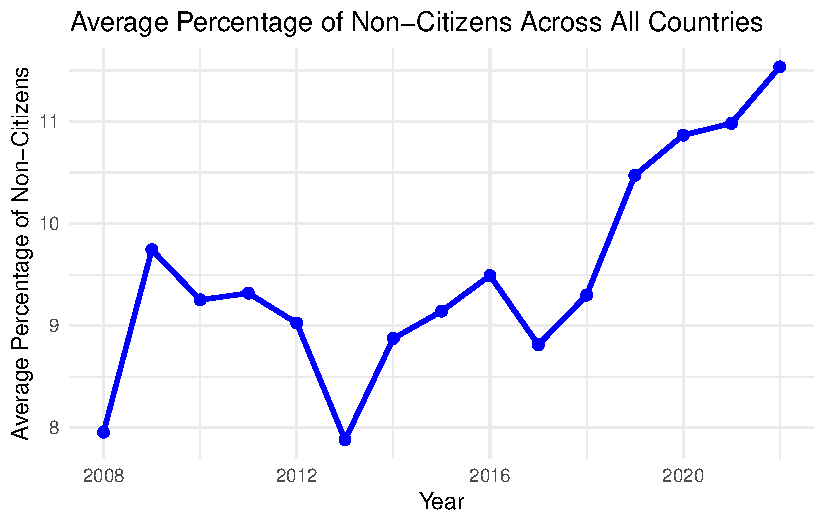
\includegraphics{DataMan_Project_files/figure-pdf/unnamed-chunk-25-1.pdf}

Figure 1: \textbf{\emph{Percentage of Non-Citizens Over Time}}

\emph{Note}: This graph tracks the proportion of non-citizens in the
population over time for selected countries. It shows a steady increase
in most countries, with Austria leading in growth, reaching 17\% by
2022. Bulgaria diverges with a declining trend, reflecting differing
demographic dynamics.

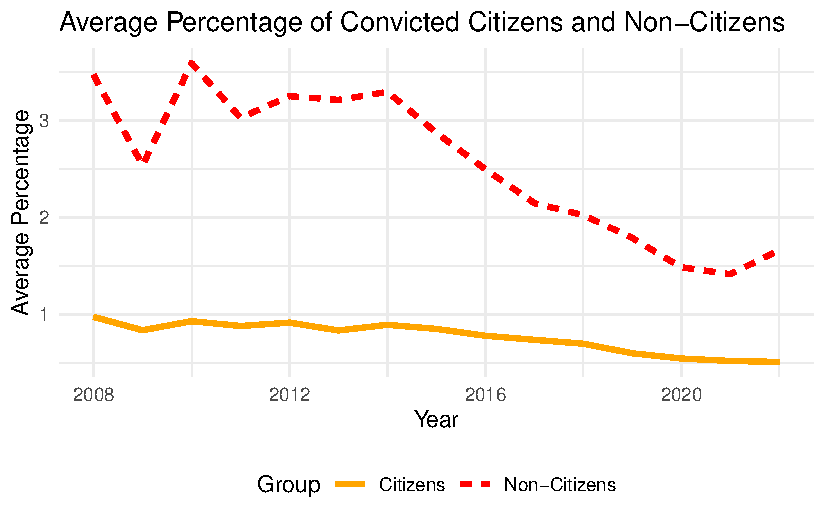
\includegraphics{DataMan_Project_files/figure-pdf/unnamed-chunk-26-1.pdf}

Figure 2: \textbf{\emph{Crime Conviction Over Time}}

\emph{Note}: This graph illustrates the number of individuals convicted
of crimes, separated by citizenship status. Non-citizens exhibit higher
conviction rates compared to citizens, with non-citizen conviction rates
declining steadily from 2008 to 2020. Citizen conviction rates start at
around 1\% and approach zero by 2022, indicating a systemic disparity in
convictions.

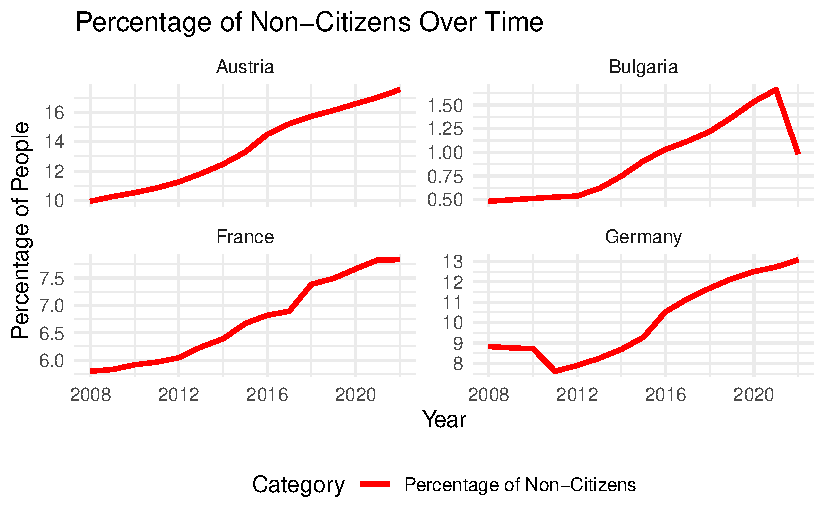
\includegraphics{DataMan_Project_files/figure-pdf/unnamed-chunk-27-1.pdf}

Figure 3: \textbf{\emph{Crime Suspicion Over Time}}

\emph{Note:} This graph shows the number of individuals suspected of
crimes, dis-aggregated by citizenship status (citizens vs.~non-citizens)
from 2008 to 2022. It highlights a significant disparity, with
non-citizens consistently suspected at higher rates than citizens. Key
trends include a notable spike in non-citizen suspicion rates in 2014,
while citizen suspicion rates remain relatively stable, averaging 0-1\%.

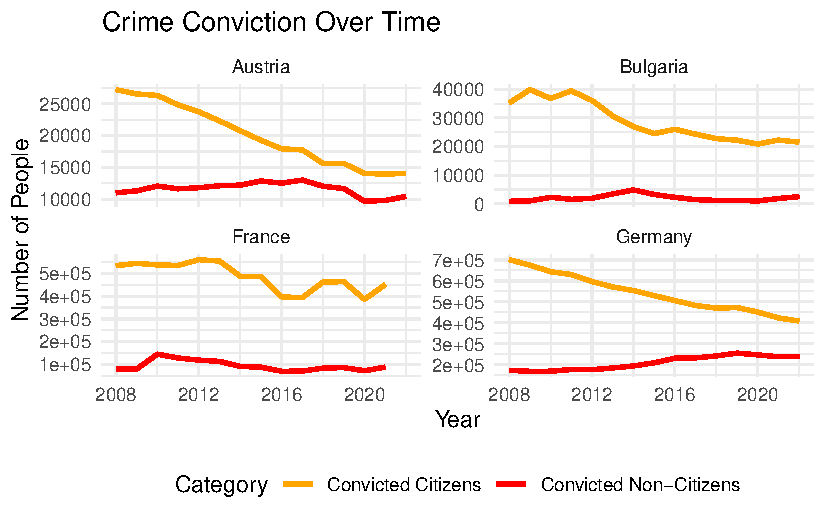
\includegraphics{DataMan_Project_files/figure-pdf/unnamed-chunk-28-1.pdf}

Figure 4: \textbf{\emph{Percentage of Non-Citizens in Selected Countries
Over Time}}

\emph{Note:} This graph shows the percentage of non-citizens relative to
the total population in four selected countries (France, Germany,
Austria, and Bulgaria) from 2008 to 2022. The trends are visualized
individually for each country, with the y-axis scaled independently to
accommodate country-specific variations. Key insights include a steady
increase in the percentage of non-citizens in most countries, with
Austria showing the most significant growth, while Bulgaria exhibits a
declining trend. This graph highlights demographic shifts in the
proportion of non-citizens, offering critical context for understanding
crime-related data.

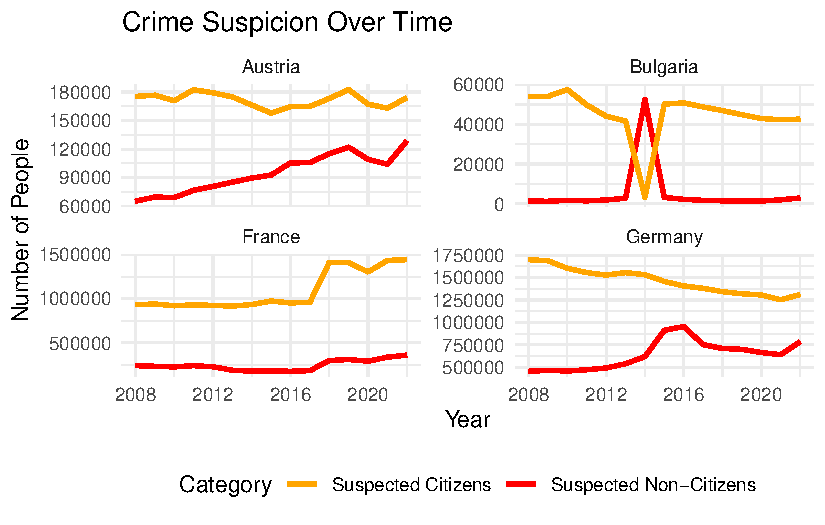
\includegraphics{DataMan_Project_files/figure-pdf/unnamed-chunk-29-1.pdf}

Figure 5: \textbf{\emph{Crime Convictions Over Time by Citizenship
Status}}

\emph{Note:} This graph illustrates the trends in crime convictions for
both non-citizens and citizens over time in selected countries. The data
is dis-aggregated by country, with each country shown in a separate
facet, and the y-axis scaled independently for better visualization of
country-specific patterns. The red line represents convictions of
non-citizens, while the orange line represents convictions of citizens.

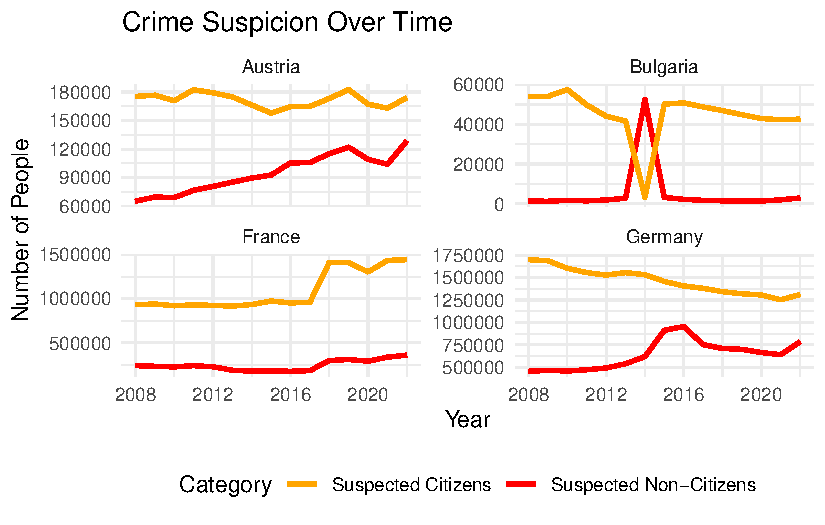
\includegraphics{DataMan_Project_files/figure-pdf/unnamed-chunk-30-1.pdf}

Figure 6: \textbf{\emph{Crime Suspicions Over Time by Citizenship
Status}}

\emph{Note:} This graph illustrates the trends in crime suspicions for
both non-citizens and citizens over time in selected countries. The data
is dis-aggregated by country, with each country shown in a separate
facet, and the y-axis scaled independently for better visualization of
country-specific patterns. The red line represents convictions of
non-citizens, while the orange line represents convictions of citizens.

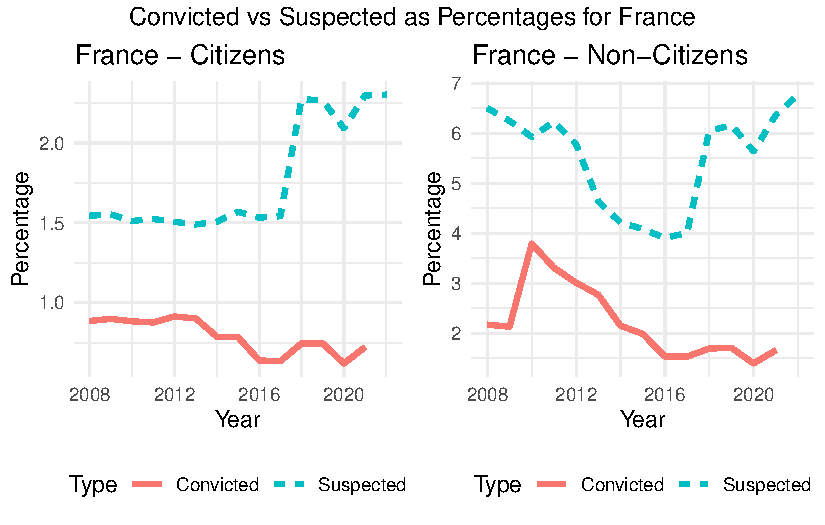
\includegraphics{DataMan_Project_files/figure-pdf/unnamed-chunk-31-1.pdf}

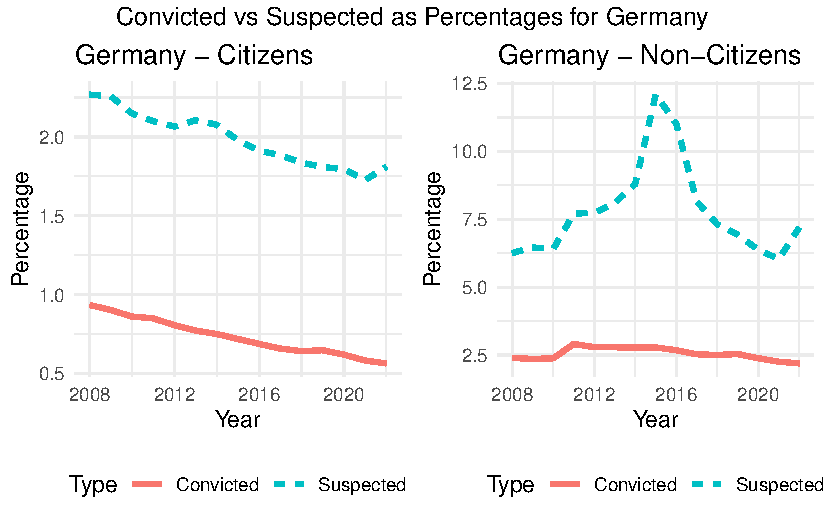
\includegraphics{DataMan_Project_files/figure-pdf/unnamed-chunk-31-2.pdf}

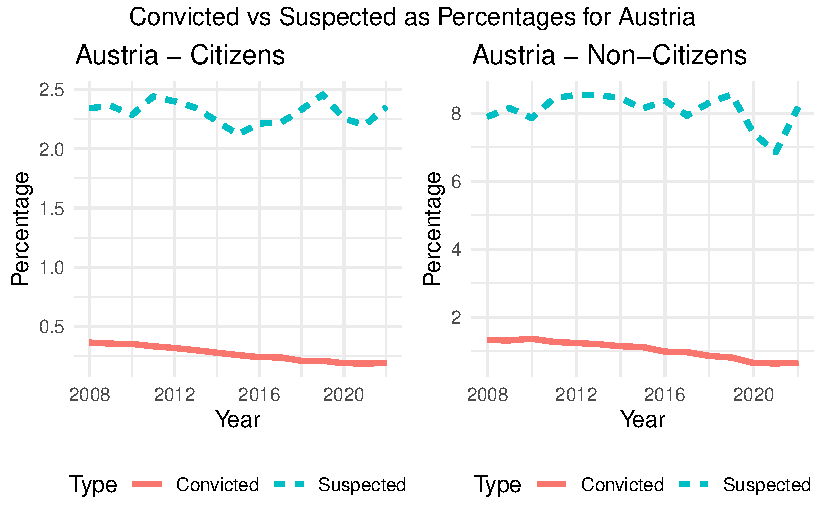
\includegraphics{DataMan_Project_files/figure-pdf/unnamed-chunk-31-3.pdf}

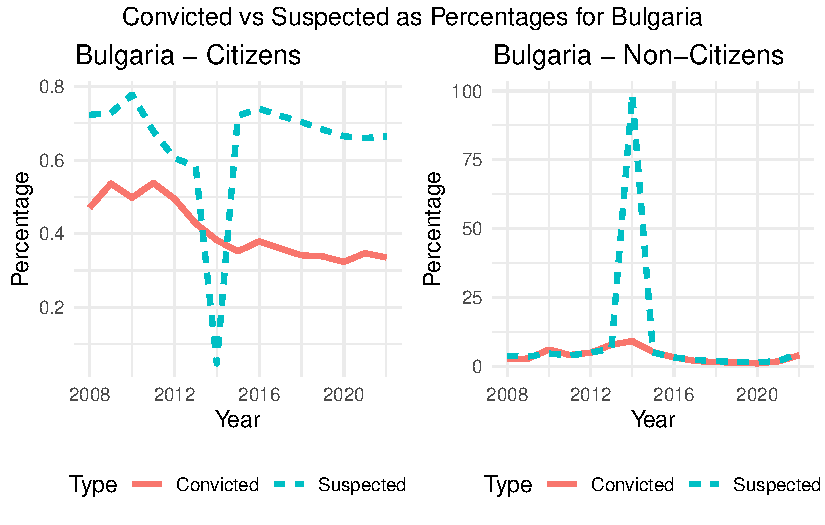
\includegraphics{DataMan_Project_files/figure-pdf/unnamed-chunk-31-4.pdf}

Figure 6: \textbf{\emph{Convicted vs.~Suspected Percentages Over Time
for Citizens and Non-Citizens}}

\emph{Note}: This series of graphs displays the trends in conviction and
suspicion rates as percentages of the respective populations (citizens
and non-citizens) for four selected countries: France, Germany, Austria,
and Bulgaria. Each country is presented in a separate panel with two
subplots. Citizens (Left Panel): Shows the average conviction and
suspicion rates for citizens over time. Non-Citizens (Right Panel):
Depicts the average conviction and suspicion rates for non-citizens over
time. The Y-axis represents the percentage of each group (citizens or
non-citizens) suspected or convicted of crimes.

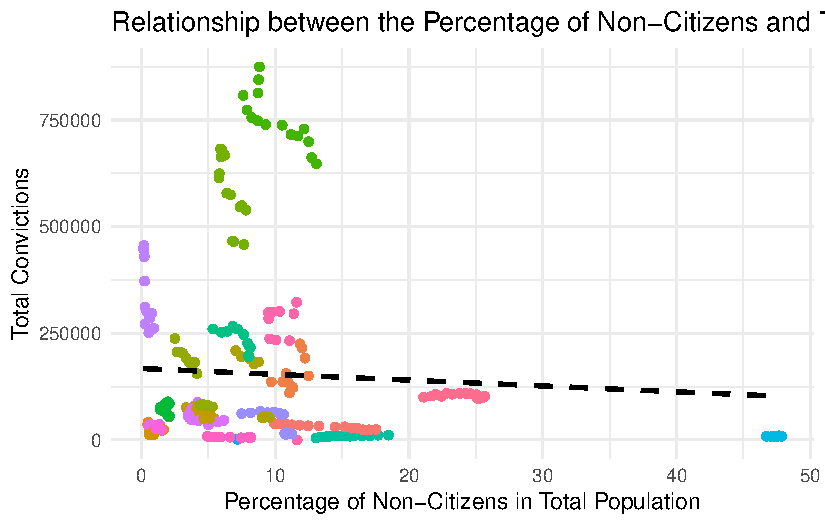
\includegraphics{DataMan_Project_files/figure-pdf/unnamed-chunk-32-1.pdf}

Figure 7: \textbf{\emph{Relationship between the Percentage of Migrants
and Total Convictions}}

\emph{Note:} This scatter plot shows the relationship between the
percentage of non-citizens in the total population and the total number
of convictions across countries. Each point represents a country in a
given year. The dashed black line represents the linear regression model
fit, showing a weak correlation between the variables, suggesting that
total convictions are not strongly driven by the percentage of
non-citizens.

\begin{table}
\centering
\caption{Regression Results: Total Convicted Persons}
\centering
\begin{tabular}[t]{l|l|r|r|r|r}
\hline
  & Term & Estimate & Std.Error & t.value & p.value\\
\hline
(Intercept) & Intercept & 167332.615 & 17607.320 & 9.504 & 0.000\\
\hline
percentage\_nc\_pop & \% Non-Citizens & -1363.033 & 1438.105 & -0.948 & 0.344\\
\hline
\end{tabular}
\end{table}

Table 1: \textbf{\emph{Regression Results for Total Convictions
(Percentage of Non-Citizens)}}

\emph{Note:} This table provides the regression results for the
relationship between total convictions and the percentage of
non-citizens. The coefficients represent the estimated effects, with
standard errors, t-values, and p-values provided to assess statistical
significance.

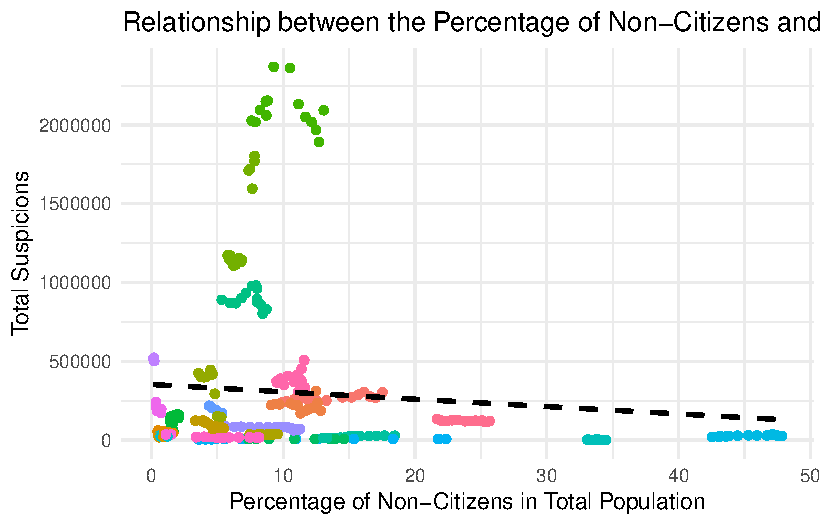
\includegraphics{DataMan_Project_files/figure-pdf/unnamed-chunk-34-1.pdf}

Figure 8: \textbf{\emph{Relationship between the Percentage of Migrants
and Total Suspicions}}

\emph{Note:} This scatter plot illustrates the relationship between the
percentage of non-citizens in the total population and the total number
of suspicions. Similar to convictions, the linear regression model
(dashed black line) indicates a weak association, with no strong
evidence that the proportion of non-citizens drives suspicion numbers.

\begin{table}
\centering
\caption{Regression Results: Total Suspected Persons}
\centering
\begin{tabular}[t]{l|l|r|r|r|r}
\hline
  & Term & Estimate & Std.Error & t.value & p.value\\
\hline
(Intercept) & Intercept & 352159.176 & 40433.52 & 8.710 & 0.000\\
\hline
percentage\_nc\_pop & \% Non-Citizens & -4670.398 & 2678.63 & -1.744 & 0.082\\
\hline
\end{tabular}
\end{table}

Table 2: \textbf{\emph{Regression Results for Total Suspicions
(Percentage of Non-Citizens)}}

\emph{Note:} This table summarizes the regression results for the
relationship between total suspicions and the percentage of
non-citizens. The provided metrics help evaluate the strength and
significance of this relationship.

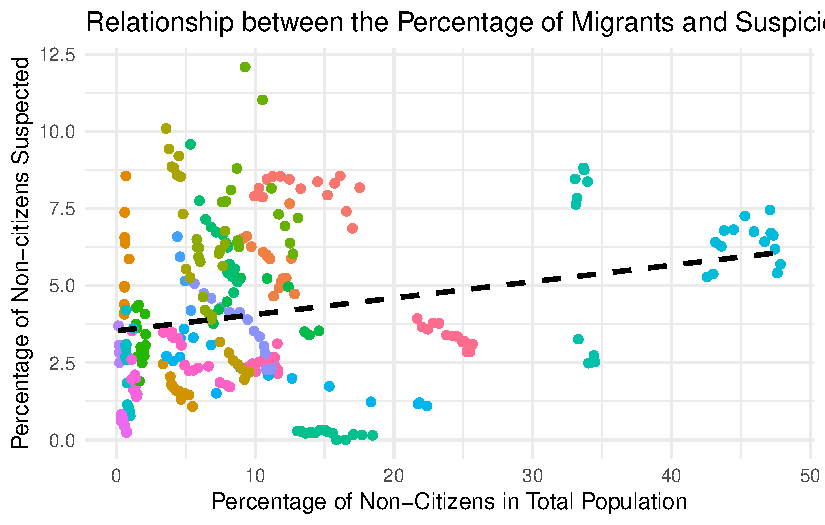
\includegraphics{DataMan_Project_files/figure-pdf/unnamed-chunk-36-1.pdf}

Figure 9: \textbf{\emph{Relationship between the Percentage of Migrants
and Suspicion Rates for Non-Citizens}}

\emph{Note:} This scatter plot focuses on the percentage of non-citizens
suspected of crimes relative to the non-citizen population. Bulgaria was
removed as an outlier. The linear regression line shows a positive
association, indicating that as the percentage of non-citizens in the
population increases, suspicion rates for non-citizens also rise.

\begin{table}
\centering
\caption{Regression Results: Total Suspected Persons}
\centering
\begin{tabular}[t]{l|l|r|r|r|r}
\hline
  & Term & Estimate & Std.Error & t.value & p.value\\
\hline
(Intercept) & Intercept & 352159.176 & 40433.52 & 8.710 & 0.000\\
\hline
percentage\_nc\_pop & \% Non-Citizens & -4670.398 & 2678.63 & -1.744 & 0.082\\
\hline
\end{tabular}
\end{table}

Table 3: \textbf{\emph{Regression Results for Non-Citizen Suspicion
Rates (Percentage of Non-Citizens)}}

\emph{Note:} The table details the regression model estimating the
effect of the percentage of non-citizens on suspicion rates for
non-citizens, excluding Bulgaria. The results highlight a statistically
significant positive relationship.

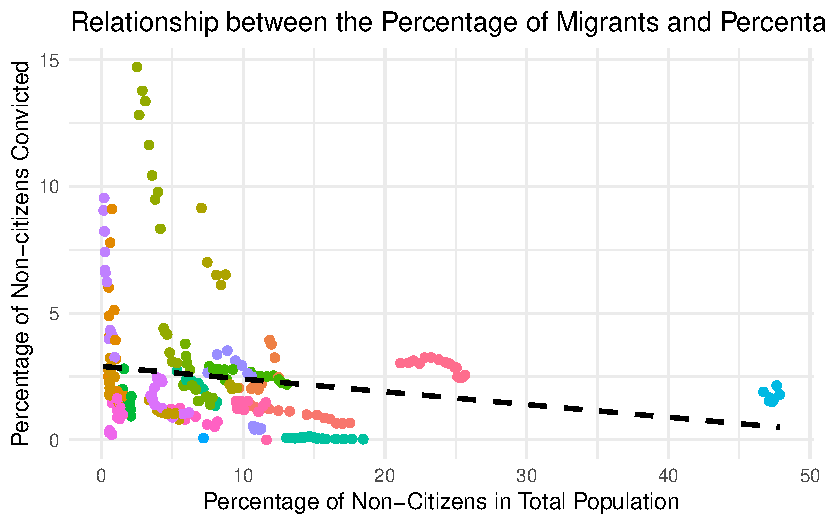
\includegraphics{DataMan_Project_files/figure-pdf/unnamed-chunk-38-1.pdf}

Figure 10: \textbf{\emph{Relationship between the Percentage of Migrants
and Conviction Rates for Non-Citizens}}

\emph{Note:} This scatter plot examines the percentage of non-citizens
convicted of crimes relative to the non-citizen population. The
regression line suggests a weaker positive correlation compared to
suspicion rates, indicating systemic factors influencing conviction
rates beyond population proportions.

\begin{table}
\centering
\caption{Regression Results: Total Convicted Persons}
\centering
\begin{tabular}[t]{l|l|r|r|r|r}
\hline
  & Term & Estimate & Std.Error & t.value & p.value\\
\hline
(Intercept) & Intercept & 2.903 & 0.208 & 13.976 & 0.000\\
\hline
percentage\_nc\_pop & \% Non-Citizens & -0.050 & 0.017 & -2.963 & 0.003\\
\hline
\end{tabular}
\end{table}

Table 4: \textbf{\emph{Regression Results for Non-Citizen Conviction
Rates (Percentage of Non-Citizens)}}

\emph{Note:} The table summarizes the regression results for non-citizen
conviction rates. The coefficients indicate the strength of the
relationship between non-citizen proportions and conviction rates, with
statistical significance levels included.

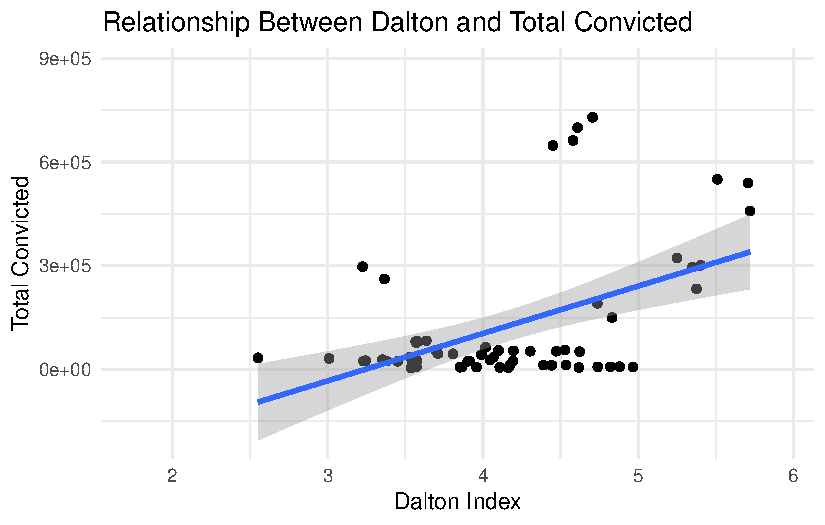
\includegraphics{DataMan_Project_files/figure-pdf/unnamed-chunk-40-1.pdf}

Figure 11: \textbf{\emph{Relationship between Polarization (Dalton
Index) and Total Convictions}}

\emph{Note:} This graph explores the impact of political polarization
(measured by the Dalton Index) on total convictions. The regression line
suggests a weak positive relationship, where higher polarization is
associated with slightly higher conviction numbers.

\begin{table}
\centering
\caption{Regression Results: Total Convicted (Polynomial Regression)}
\centering
\begin{tabular}[t]{l|l|r|r|r|r}
\hline
  & Term & Estimate & Std.Error & t.value & p.value\\
\hline
(Intercept) & Intercept & -4956.102 & 968373.49 & -0.005 & 0.996\\
\hline
dalton & Dalton Index & 138249.609 & 31731.63 & 4.357 & 0.000\\
\hline
poly(year, 2)1 & Year (Polynomial Term 1) & -8507919.553 & 19191744.90 & -0.443 & 0.659\\
\hline
poly(year, 2)2 & Year (Polynomial Term 2) & 2680583.326 & 6918733.52 & 0.387 & 0.700\\
\hline
\end{tabular}
\end{table}

Table 5: \textbf{\emph{Regression Results for Total Convictions (Dalton
Index)}}

\emph{Note:} The table presents the polynomial regression results,
including quadratic terms for the year. The Dalton Index shows a small
but statistically significant association with total convictions.

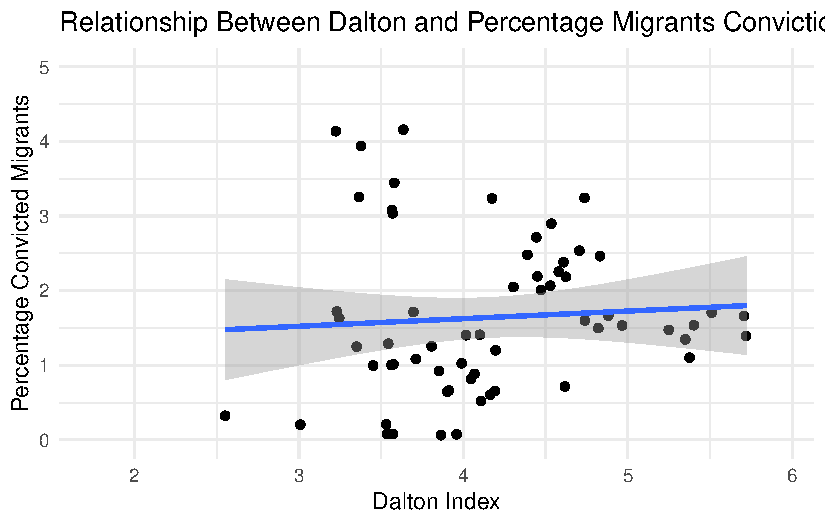
\includegraphics{DataMan_Project_files/figure-pdf/unnamed-chunk-42-1.pdf}

Figure 12: \textbf{\emph{Relationship between Polarization and
Percentage of Migrants Convicted}}

\emph{Note:} This graph examines the effect of political polarization on
conviction rates for non-citizens. The regression line shows a weak
positive association, suggesting that polarization might play a role in
conviction outcomes for non-citizens.

\begin{table}
\centering
\caption{Regression Results: Convicted Non-Citizens (Polynomial Regression)}
\centering
\begin{tabular}[t]{l|l|r|r|r|r}
\hline
  & Term & Estimate & Std.Error & t.value & p.value\\
\hline
(Intercept) & Intercept & 8.734 & 5.884 & 1.484 & 0.143\\
\hline
dalton & Dalton Index & 0.127 & 0.193 & 0.658 & 0.513\\
\hline
poly(year, 2)1 & Year (Polynomial Term 1) & -149.479 & 116.609 & -1.282 & 0.205\\
\hline
poly(year, 2)2 & Year (Polynomial Term 2) & 52.366 & 42.038 & 1.246 & 0.218\\
\hline
\end{tabular}
\end{table}

Table 6: \textbf{\emph{Regression Results for Non-Citizen Conviction
Rates (Dalton Index)}}

\emph{Note:} This table summarizes the regression results for the
relationship between the Dalton Index and conviction rates for
non-citizens, highlighting the significance of polarization in shaping
judicial outcomes.

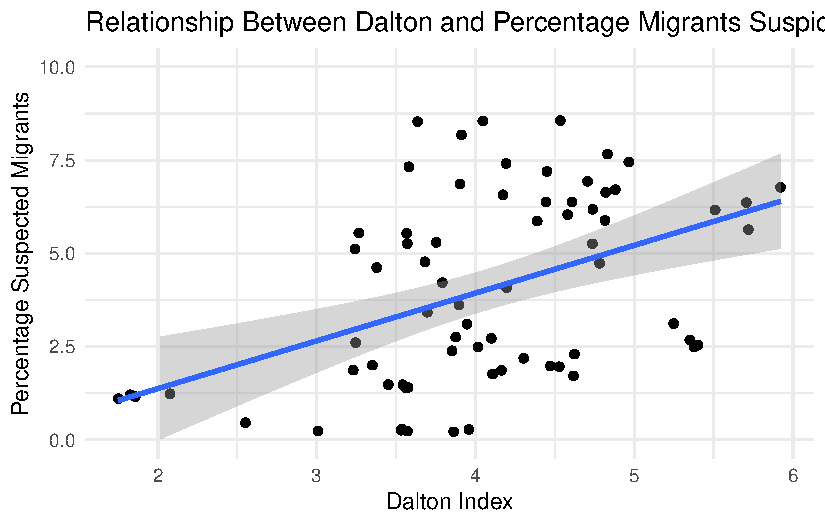
\includegraphics{DataMan_Project_files/figure-pdf/unnamed-chunk-44-1.pdf}

Figure 13: \textbf{\emph{Relationship between Polarization and
Percentage of Migrants Suspected}}

\emph{Note:} This graph investigates the association between political
polarization and suspicion rates for non-citizens. The positive trend in
the regression line indicates that higher polarization correlates with
increased suspicion rates for non-citizens.

\begin{table}
\centering
\caption{Regression Results: Suspected Non-Citizens (Polynomial Regression)}
\centering
\begin{tabular}[t]{l|l|r|r|r|r}
\hline
  & Term & Estimate & Std.Error & t.value & p.value\\
\hline
(Intercept) & Intercept & 6.023 & 12.072 & 0.499 & 0.619\\
\hline
dalton & Dalton Index & 1.284 & 0.311 & 4.129 & 0.000\\
\hline
poly(year, 2)1 & Year (Polynomial Term 1) & -144.700 & 237.297 & -0.610 & 0.544\\
\hline
poly(year, 2)2 & Year (Polynomial Term 2) & 54.725 & 85.133 & 0.643 & 0.523\\
\hline
\end{tabular}
\end{table}

Table 7: \textbf{\emph{Regression Results for Non-Citizen Suspicion
Rates (Dalton Index)}}

\emph{Note:} This table provides the polynomial regression results for
the relationship between the Dalton Index and suspicion rates for
non-citizens. The significant positive relationship suggests that
polarization affects suspicion outcomes.

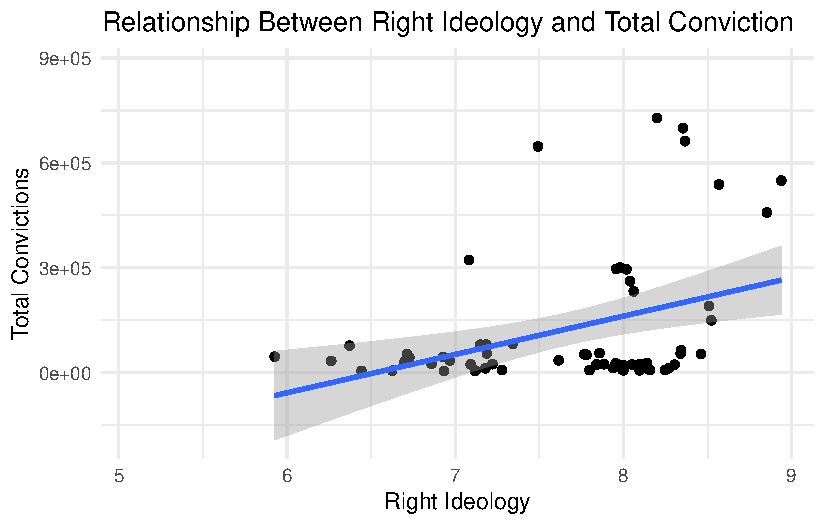
\includegraphics{DataMan_Project_files/figure-pdf/unnamed-chunk-46-1.pdf}

Figure 14: \textbf{\emph{Relationship between Right Ideology and Total
Convictions}}

\emph{Note:} This graph examines the influence of right-wing ideology on
total convictions. The regression line shows a weak positive
relationship, suggesting that stronger right-wing ideology is not a
major driver of total convictions.

\begin{table}
\centering
\caption{Regression Results: Total Convicted (Right-Wing Ideology)}
\centering
\begin{tabular}[t]{l|l|r|r|r|r}
\hline
  & Term & Estimate & Std.Error & t.value & p.value\\
\hline
(Intercept) & Intercept & -40543708.9 & 47264753.74 & -0.858 & 0.394\\
\hline
right\_ideology & Right-Wing Ideology & 123308.6 & 37615.69 & 3.278 & 0.002\\
\hline
year & Year & 19661.5 & 23331.92 & 0.843 & 0.403\\
\hline
\end{tabular}
\end{table}

Table 8: \textbf{\emph{Regression Results for Total Convictions
(Right-Wing Ideology)}}

\emph{Note:} The table summarizes the regression results for total
convictions, considering right-wing ideology and year as predictors. The
results provide insight into the relationship between ideological trends
and crime outcomes.

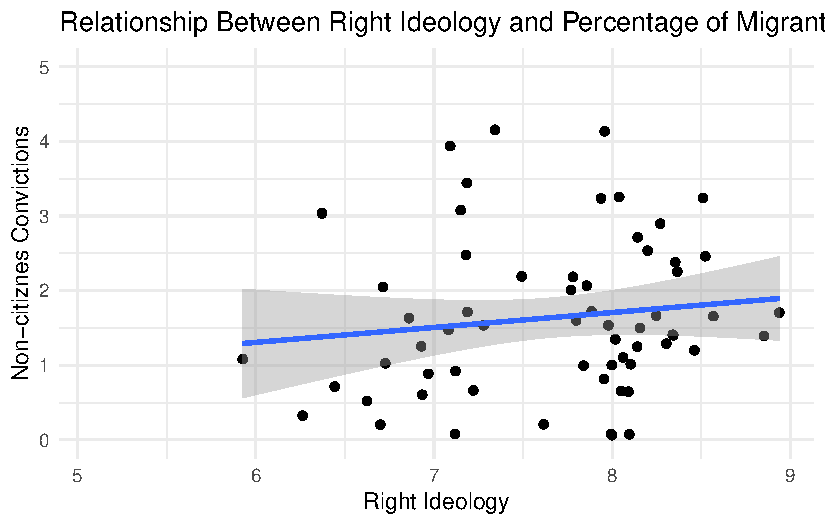
\includegraphics{DataMan_Project_files/figure-pdf/unnamed-chunk-48-1.pdf}

Figure 15: \textbf{\emph{Relationship between Right Ideology and
Conviction Rates for Non-Citizens}}

\emph{Note:} This graph focuses on conviction rates for non-citizens and
their relationship with right-wing ideology. The weak positive
correlation implies a limited influence of ideology on conviction
outcomes.

\begin{table}
\centering
\caption{Regression Results: Convicted Non-Citizens (Right-Wing Ideology)}
\centering
\begin{tabular}[t]{l|l|r|r|r|r}
\hline
  & Term & Estimate & Std.Error & t.value & p.value\\
\hline
(Intercept) & Intercept & 12.314 & 273.398 & 0.045 & 0.964\\
\hline
right\_ideology & Right-Wing Ideology & 0.196 & 0.218 & 0.901 & 0.371\\
\hline
year & Year & -0.006 & 0.135 & -0.045 & 0.965\\
\hline
\end{tabular}
\end{table}

Table 9: \textbf{\emph{Regression Results for Non-Citizen Conviction
Rates (Right-Wing Ideology)}}

\emph{Note:} This table provides regression results for the relationship
between right-wing ideology and non-citizen conviction rates. The
coefficients highlight whether ideological trends significantly affect
judicial outcomes.

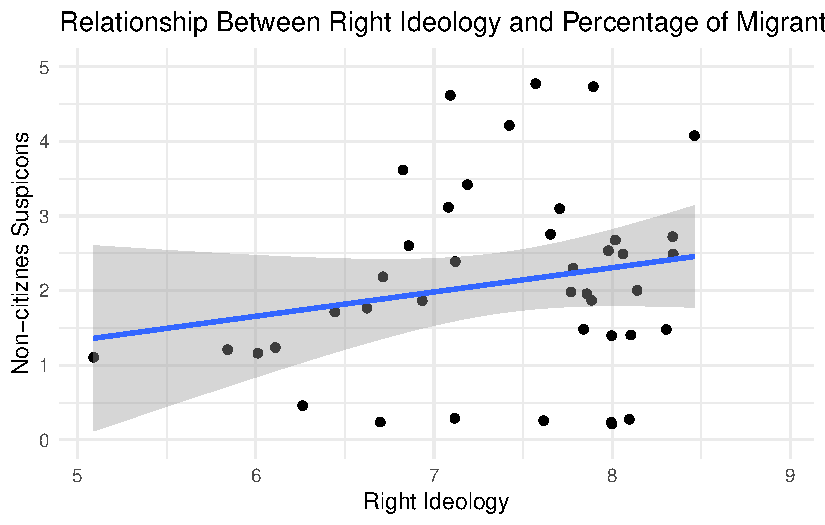
\includegraphics{DataMan_Project_files/figure-pdf/unnamed-chunk-50-1.pdf}

Figure 16: \textbf{\emph{Relationship between Right Ideology and
Suspicion Rates for Non-Citizens}}

\emph{Note:} This graph investigates the relationship between right-wing
ideology and suspicion rates for non-citizens. The regression line
indicates a stronger positive correlation, suggesting that suspicion
rates are more sensitive to ideological shifts.

\begin{table}
\centering
\caption{Regression Results: Suspected Non-Citizens (Right-Wing Ideology)}
\centering
\begin{tabular}[t]{l|l|r|r|r|r}
\hline
  & Term & Estimate & Std.Error & t.value & p.value\\
\hline
(Intercept) & Intercept & -872.930 & 541.437 & -1.612 & 0.112\\
\hline
right\_ideology & Right-Wing Ideology & 1.387 & 0.391 & 3.551 & 0.001\\
\hline
year & Year & 0.429 & 0.267 & 1.603 & 0.114\\
\hline
\end{tabular}
\end{table}

Table 10: \textbf{\emph{Regression Results for Non-Citizen Suspicion
Rates (Right-Wing Ideology)}}

\emph{Note:} This table summarizes the regression results for the
relationship between right-wing ideology and suspicion rates for
non-citizens, showing significant associations.




\end{document}
